
\section{Die Entdeckung des Gluons}

\chapterauthor{Dominik Hellmann, 09.11.2018}

\subsection{Theoretische Grundlagen der Quantenchromodynamik}
Die Quantenchromodynamik (QCD) ist die Quantenfeldtheorie der starken Wechselwirkung, d.h. der Kraft, die für das Zusammenhalten der Quarks in Hadronen verantwortlich ist.
Grundlage für die QCD ist die Yang-Mills-Theorie, welche eine im Jahre 1954 entwickelte Eichtheorie ist.
Dabei folgt die QCD aus der $SU(3)_\text{c}$-Symmetriegruppe, wobei hieraus die drei Farbladungen rot, grün, blau und die dazugehörigen Antifarben resultieren.
Die Farben sind dabei analog zu den elektrischen Ladungen der QED zu verstehen.

Analog zu den Photonen der QED existieren auch Eichbosonen der QCD, welche Gluonen heißen.
Aus der Gruppentheorie folgt, dass 8 Gluonen existieren, welche den Generatoren der $SU(3)_\text{c}$ entsprechen.
Gluonen sind masselose Vektorteilchen, welche jedoch im Kontrast zur QED ebenfalls Farbladung besitzen und dementsprechend an sich selbst koppeln können.
Hieraus folgt die asymptotische Freiheit als charakteristische Eigenschaft der QCD:
Durch Vakuumpolarisationen, dem sogenannten Anti-Screening, wird die Kopplungskonstante der QCD $\alpha_{s}$ klein für große Impulsüberträge. 
Hieraus folgt, dass die einzelnen Quarks bei großen Impulsüberträgen, bzw. kleinen Abständen, als asymptotisch frei verstanden werden können.
Andererseits folgt als Charakteristikum das Confinement: Bei großen Abständen steigt das Potential der QCD linear an, d.h. die Kraft für das weitere Vergrößern des Abstandes wächst linear.
Wird der Abstand weiter vergrößert, so werden neue Teilchen in sogenannten Jets produziert, bis der Endzustand wieder farbneutral ist.
Dementsprechend können farbgeladene Teilchen nur in einem farbneutralen, gebundenen Zustand beobachtet werden.
Die entstehenden Jets können in einem Detektor als Ansammlung von Teilchen beobachtet werden, wobei die Messung der Impulse aller beobachteten Teilchen Rückschlüsse auf die Impulse der ursprünglichen Quarks zulässt.

\subsection{Historische Entwicklung}

Im Jahr 1964 wurden von Murray Gell-Mann erstmals Quarks als Bestandteile der Hadronen postuliert.
Hierbei stellen sich die Fragen, welche Kräfte diese Elementarteilchen zusammenhalten und welche Austauschteilchen diese Kraft vermitteln.
Weitere Hinweise auf eine mit der QCD verbundenen Quantenzahl stellten die $\Delta$-Baryonen sowie der $R$-Plot dar.
So ist die Wellenfunktion des $\Delta^{++}$-Baryons unter Vertauschung von zwei Quarks symmetrisch, falls nur die bisher bekannten Raum-, Flavour- und Spinanteile der Wellenfunktion berücksichtigt werden.
Dies steht jedoch im Widerspruch mit dem Pauliprinzip für Fermionen.
Die Einführung einer Farbe als Quantenzahl stellt den nötigen antisymmetrischen Anteil der Wellenfunktion bereit und löst somit dieses Problem.

Bei der Betrachtung des $R$-Plots wird die Häufigkeit der Produktion von Hadronen in $e^+ e^-$ Reaktionen in Abhängigkeit von der Schwerpunktsenergie betrachtet.
Hierbei ist das Verhältnis $R$ sensitiv auf das Vorhandensein von Farbladungen und sagt experimentell drei Farbladungen voraus.

\subsection{Jetphysik am DESY}
Das DESY (Deutsche Elektron Synchrotron) ist ein Forschungszentrum für Teilchenphysik, welches 1959 in Hamburg gegründet wurde.
Der dort gebaute $e^+ e^-$ Collider PETRA (Positron-Electron-Tandem-Ring Accelerator) wurde im Oktober 1978 in Betrieb genommen.
Mit einem Umfang von $U=\SI{2.3}{\kilo\metre}$ konnten im späteren Betrieb Schwerpunktsenergien von bis zu $\SI{47}{\giga\electronvolt}$ erreicht werden.
Eines der an diesem Collider arbeitenden Experimente war TASSO (Two Arm Spectrometer Solenoid).
Mithilfe des mit einem Magnetfeld durchsetzten Zentraldetektors war eine genaue Impulsmessung möglich, zur Geschwindigkeitsmessung wurde ein Flugzeitzählersystem verwendet.
In den beiden Armen des Detektors konnte durch drei Lagen von Schwellen-Cherenkovzählern, Schauerzählern sowie den Flugzeitzählersystemen eine sehr gute Teilchenidentifikation ermöglicht werden.

Die Jet-Rekonstruktion zu dieser Zeit konzentrierte sich insbesondere auf die Beobachtung von 2-Jet-Ereignissen, wie sie 1975 durch Feynman erstmals vorhergesagt und 1978 am DESY entdeckt wurden.
Im Rahmen des Cone-Algorithmus wird dabei eine Hauptjetachse gesucht und die Impulse entlang dieser Achse maximiert beziehungsweise die Impulse transversal zu der Hauptachse minimiert.
Um die Existenz von Gluonen in der QCD zu beweisen kann das Auftreten von 3-Jet-Strukturen verwendet werden.
Dies entspricht der Abstrahlung eines Gluons, wie in Abbildung \ref{fig:gluon} dargestellt ist.
\begin{figure}
  \centering
  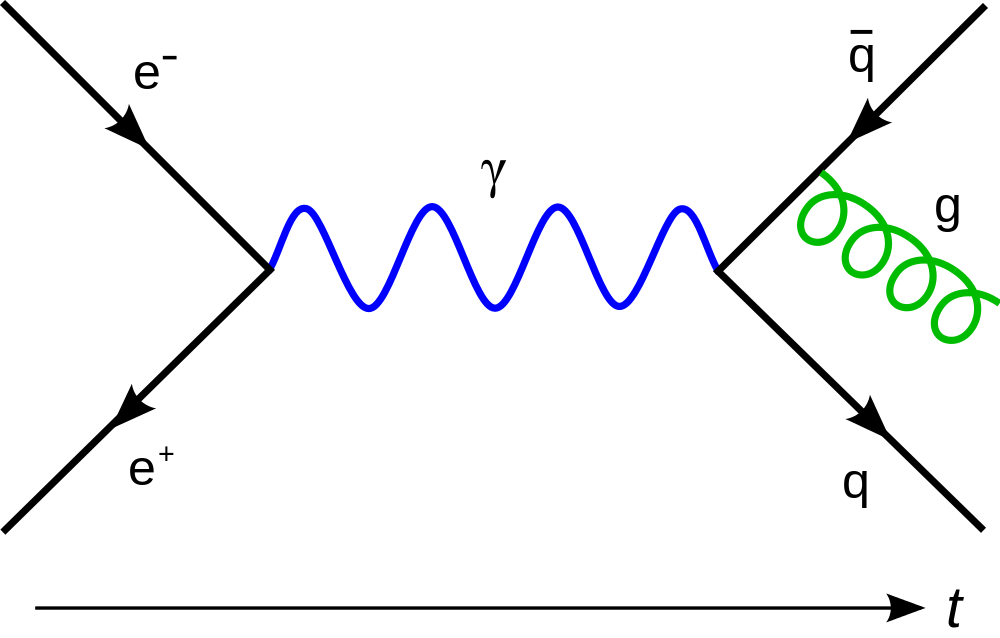
\includegraphics[height=4.0cm]{ressources/gluon.png}
  \caption{Abstrahlung eines Gluons in einer $e^+ e^-$-Kollision \cite{gluon}.}
  \label{fig:gluon}
\end{figure}
Bei einem ausreichend großen Transversalimpuls des Gluons entsteht ein dritter Jet, der im Detektor nachgewiesen werden kann.

\subsection{Analyse der Jets der TASSO-Kollaboration}
Die Analyse der Jets wurde von der TASSO-Kollaboration bei verschiedenen Schwerpunktsenergien durchgeführt. 
Dabei teilt sich die Analyse jeweils in verschiedene Schritte auf.
Zunächst wird die Hauptjetachse durch das Maximieren des Impulses in die Jetachsenrichtung bestimmt.
Die Verteilung der Impulse transversal zur Hauptachse wird nun untersucht, wobei hier einer energieabhängige Verteilung der Transveralimpulse beobachtet wurde, die mit der Schwerpunktsenergie zugenommen hat. 
Dies widerspricht den bisherigen naiven Partonmodellen und ließe sich beispielsweise über die Abstrahlung von Gluonen erklären.

Im nächsten Schritt werden die Breiten der einzelnen Jets untersucht.
Bei zwei rekonstruierten Jets wäre zu erwarten, dass jeweils nur ein Jet aufgrund von Gluonabstrahlung verbreitert ist und somit eine Asymmetrie zu beobachten ist.
Die Ergebnisse zeigen, dass die Asymmetrie für größere Schwerpunktsenergien ansteigt und somit für verschiedene Energien unterschiedliche Parameter der Quark-Parton-Modelle verwendet werden müssen.
Auch dieses Verhalten ist mit der Abstrahlung von Gluonen als Erklärung kompatibel.

Der letzte Schritt besteht darin, die Struktur der 3-Jet-Ereignisse eindeutig von den kollinearen 2-Jet-Ereignissen zu trennen.
Dabei müssen die drei beobachteten Jets aufgrund der Impulserhaltung in einer Ebene liegen, jedoch eine Abweichung von der kollinearen Struktur innerhalb dieser Ebene aufweisen.
Dazu wird aus den beobachteten Impulsen der Hadron-Impulstensor ermittelt.
Aus den Eigenvektoren dieses Tensors lassen sich die Größen $\left<p_T^2\right>_\text{in}$ und $\left<p_T^2\right>_\text{out}$ ermitteln welche jeweils angeben, wie stark die gemessenen Impulse aus der Ereignisebene herausragen bzw. wie stark die Impulse von der Hauptjetachse in der Ereignisebene abweichen.
Beobachtet wird, dass $\left<p_T^2\right>_\text{out}$ lediglich einen geringen Anstieg mit der Schwerpunktsenergie aufzeigt, während sich $\left<p_T^2\right>_\text{in}$ bei höheren Energien nicht mehr korrekt mit dem naiven Quark-Parton Modell beschreiben lässt.
Dies deutet auf ein drittes farbgeladenes Teilchen im Endzustand, welches bei höheren Energien einen Jet erzeugt, wobei die Häufigkeit dieser Ereignisse nicht mehr mit statistischen Fluktuationen kompatibel ist.

Der somit bestätigten Existenz des Gluons folgte die Bestimmung seines Spins, welches laut Theorie den Wert $1$ besitzen sollte.
Als hiermit korrelierte Größe wurde 1980 der sogenannte Ellis-Karliner Winkel von der TASSO-Kollaboration gemessen und mit Simulationen für verschiedene Spins des Gluons verglichen.
Hierbei wurde eine gute Übereinstimmung mit der Annahme eines Vektorteilchens, d.h. Spin 1 des Gluons, ermittelt.
Es folgten weitere Spinmessungen der SLD Kollaboration, die dieses Ergebnis bestätigten.

\subsection{Heutige Jetphysik und QCD-Forschung}

In der heutigen Jetphysik können in einem Ereignis aufgrund der höheren Schwerpunktsenergien der Beschleuniger deutlich mehr als zwei Jets beobachtet werden.
Hierzu werden effiziente und schnelle Rekonstruktionsalgorithmen benötigt, welche die Eigenschaften der Infrarot-Stabilität sowie der kollinearen Stabilität erfüllen müssen.
Dafür werden, im Vergleich zu den vorher verwendeten Cone-Algorithmen, heutzutage häufig sequentielle Cluster Algorithmen (beispielsweise $k_t$, anti-$k_t$ und Cambridge/Aachen) verwendet.

Aktuelle Forschungsfragen der QCD sind beispielsweise die Existenz von Glueballs oder der Beitrag der Gluonen und verschiedenen Quarks zum Protonspin.

\subsection{Diskussion}
Im Anschluss des Vortrages wurde gefragt, inwiefern sich die unterschiedlichen Spinmessungen des Gluons der verschiedenen Kollaborationen unterschieden haben.
Beim Folgeexperiment der SLD Kollaboration wurde durch höhere Schwerpunktsenergien und einen besseren Detektor eine höhere Auflösung und somit eine genauere Messung ermöglicht.

Zudem wurde gefragt, ob andere Kandidaten neben der QCD zur Erklärung der starken Wechselwirkung existierten.
Zwar wäre es möglich gewesen, einige Ergebnisse der Experimente zur Suche nach Gluonen durch einen weiteren Quarkflavour zu erklären - dies wurde jedoch bereits früh durch andere Experimente bei den geringen, hier genutzten Schwerpunktsenergien ausgeschlossen.
Eine generelle alternative theoretische Erklärung der starken Wechselwirkung existierte jedoch nicht.